\documentclass[tikz,border=7pt]{standalone}
\usepackage{amsmath,amssymb}
\usetikzlibrary{arrows.meta}
\definecolor{realpoint}{RGB}{158,45,49}
\definecolor{complexpoint}{RGB}{47,101,153}
\begin{document}
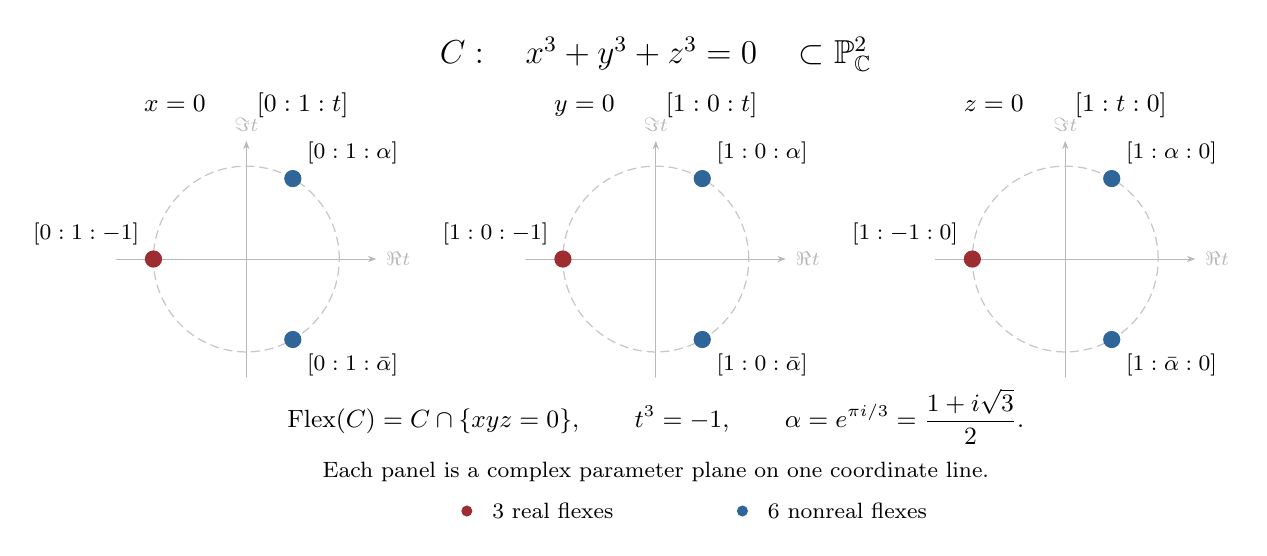
\begin{tikzpicture}[x=1cm,y=1cm,line cap=round,
    pointlabel/.style={font=\footnotesize,inner sep=2pt},
    axis/.style={black!28,line width=.35pt,-{Stealth[length=3pt]}},
    realflex/.style={circle,fill=realpoint,inner sep=2.2pt},
    complexflex/.style={circle,fill=complexpoint,inner sep=2.2pt}]
\node[font=\large] at (5.2,2.6) {$C:\quad x^3+y^3+z^3=0\quad\subset\mathbb P^2_{\mathbb C}$};
% These are complex parameter planes for the three projective coordinate
% lines, NOT three real-plane drawings of the cubic.
\foreach \shift/\heading/\param in
 {0/{x=0}/{[0:1:t]},5.2/{y=0}/{[1:0:t]},10.4/{z=0}/{[1:t:0]}}{
 \begin{scope}[shift={(\shift,0)}]
  \node[font=\small] at (0,1.95) {$\heading\qquad\param$};
  \draw[axis] (-1.65,0)--(1.65,0) node[right,font=\scriptsize] {$\Re t$};
  \draw[axis] (0,-1.5)--(0,1.5) node[above,font=\scriptsize] {$\Im t$};
  \draw[black!22,line width=.45pt,densely dashed] (0,0) circle[radius=1.18cm];
  \node[realflex] at (-1.18,0) {};
  \node[complexflex] at (.59,1.02191) {};
  \node[complexflex] at (.59,-1.02191) {};
 \end{scope}
}
\node[pointlabel,above left=3pt] at (-1.18,0) {$[0:1:-1]$};
\node[pointlabel,above right=3pt] at (.59,1.02191) {$[0:1:\alpha]$};
\node[pointlabel,below right=3pt] at (.59,-1.02191) {$[0:1:\bar\alpha]$};
\node[pointlabel,above left=3pt] at (4.02,0) {$[1:0:-1]$};
\node[pointlabel,above right=3pt] at (5.79,1.02191) {$[1:0:\alpha]$};
\node[pointlabel,below right=3pt] at (5.79,-1.02191) {$[1:0:\bar\alpha]$};
\node[pointlabel,above left=3pt] at (9.22,0) {$[1:-1:0]$};
\node[pointlabel,above right=3pt] at (10.99,1.02191) {$[1:\alpha:0]$};
\node[pointlabel,below right=3pt] at (10.99,-1.02191) {$[1:\bar\alpha:0]$};
\node[font=\small] at (5.2,-2.0)
 {$\operatorname{Flex}(C)=C\cap\{xyz=0\},\qquad
   t^3=-1,\qquad \alpha=e^{\pi i/3}=\dfrac{1+i\sqrt3}{2}.$};
\node[font=\footnotesize] at (5.2,-2.7)
 {Each panel is a complex parameter plane on one coordinate line.};
\fill[realpoint] (2.8,-3.2) circle[radius=2pt];
\node[anchor=west,font=\footnotesize] at (3,-3.2) {3 real flexes};
\fill[complexpoint] (6.3,-3.2) circle[radius=2pt];
\node[anchor=west,font=\footnotesize] at (6.5,-3.2) {6 nonreal flexes};
\end{tikzpicture}
\end{document}
